\documentclass[11pt, a4paper]{article}
\usepackage[spanish]{babel}
\usepackage[T1]{fontenc}
\usepackage[UTF8]{inputenc}
\usepackage{graphicx, amsmath, booktabs, latexsym, mathrsfs, amssymb, amsthm, units, siunitx, textcomp,subcaption,wrapfig,enumerate}
\usepackage{anysize}
\marginsize{1.5cm}{2cm}{1.5cm}{2cm}

\begin{document}
\title{Uso de motores y servos en Robótica \\ {\Large Robótica y Mecatrónica}}
\author{Arcadi Garcia, Melodía Moya} \date{}
\maketitle

\section{Cuestiones a realizar}
	\subsection{Sesión 1}
	\subsubsection{Motores DC}
		\begin{enumerate}[(a)]
			\item \textbf{Antes de montar el circuito L293B, alimente el motor con diversos voltajes (varíe el voltaje suministrado entre 3 y 5 V). Compruebe si es capaz de variar la velocidad del motor y el torque que es capaz de producir}.
			
			Tras variar el voltaje que se suministraba al motor, se observó un cambio en la velocidad de giro. A mayor tensión, mayor velocidad de giro.
			\item \textbf{Compruebe que al cambiar la polaridad del motor el giro se invierte.}.
			
			Efectivamente, el giro se invierte.
			\item \textbf{Realice el montaje del L293B y observe que puede cambiar el sentido de giro del motor.}
	
			El montaje funciona a la perfección y se puede controlar el sentido de giro del motor con un interruptor.
			
			\item \textbf{Realice un esquema de conexión para ser utilizado con un microcontrolador como la RaspBerry Pi. Conéctelo y controle el sentido del motor DC con la RaspBerry.}
			
			He aquí el montaje:
			
			\begin{figure}[h]
				\begin{center}
					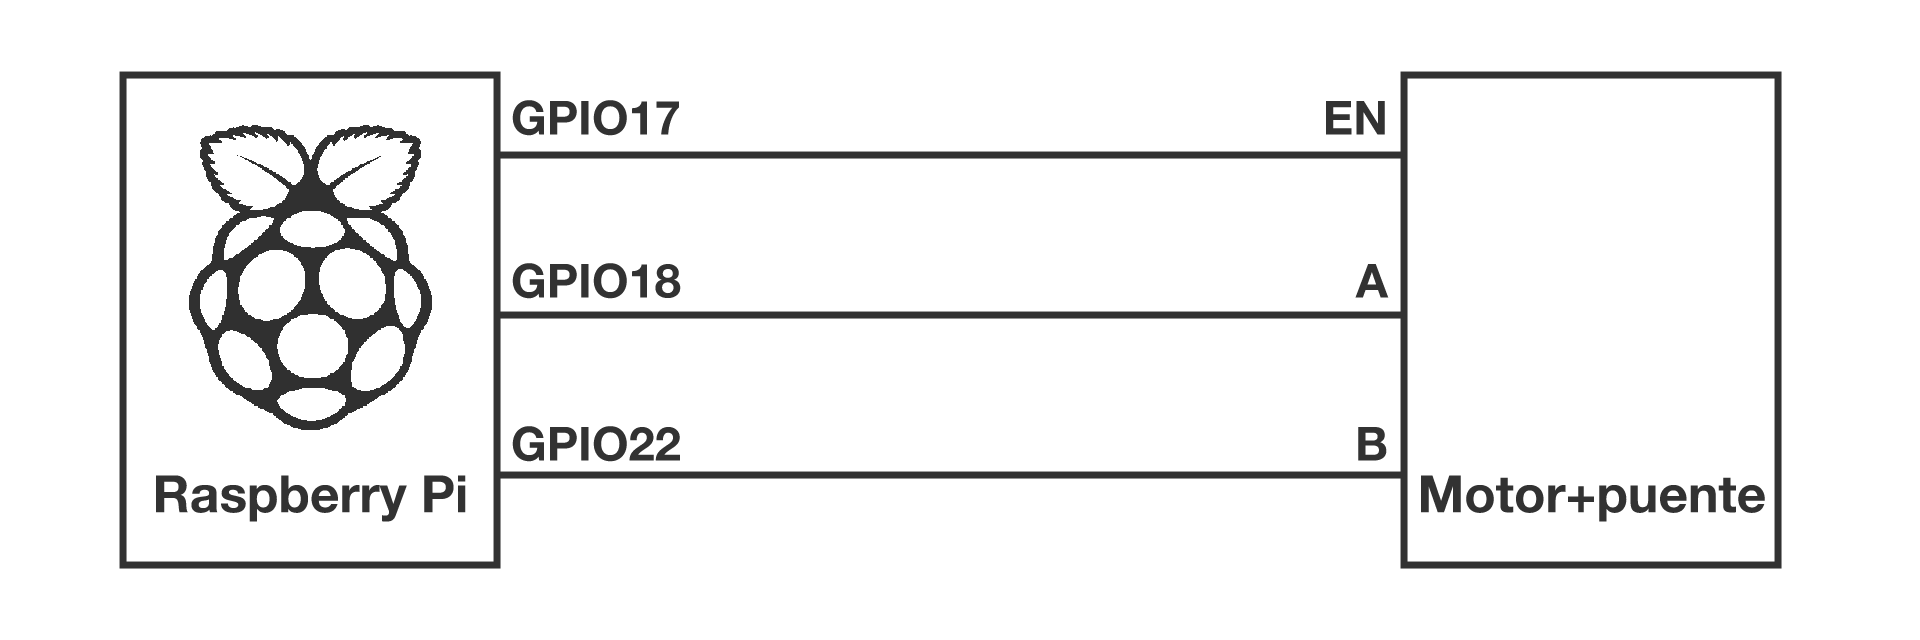
\includegraphics[width=.9\textwidth]{dcmon}
					\caption*{Esquema de conexión entre la Raspberry y la circuitería del motor. EN corresponde a la entrada de habilitación del circuito y A y B son los que determinan el sentido de giro del motor.}
				\end{center}
			\end{figure}
			
			Y el código para controlarlo:
			\begin{verbatim}
				#include <wiringPi.h>
				#include <stdio.h>
				#define DC_EN 0 //pin para el enable
				#define DC_A 1 //pines A y B para controlar el sentido de giro
				#define DC_B 3
				
				int main(){
					
					int giro=-1; //variable para escoger el sentido de giro
					
					wiringPiSetup();
					pinMode(DC_EN,OUTPUT);
					pinMode(DC_A,OUTPUT);
					pinMode(DC_B,OUTPUT);
				
					printf("Escoja sentido de giro: izquierda (0) o derecha (1)\n");
					while(giro<0 || giro>1){
						scanf("%d",&giro);
				
						if(giro<0 || giro>1){
							printf("Hágame usted el favor de introducir 0 ó 1.\n\n");
						}
					}
				    
				    //Sea como sea, encendemos el motor
				    digitalWrite(DC_EN,HIGH);
				    
				    //Y luego ya vemos en qué sentido hacerlo girar.
				    if(giro==0) {
								digitalWrite(DC_A,LOW);
								digitalWrite(DC_B,HIGH);
				    } else if(giro==1){
								digitalWrite(DC_A,HIGH);
								digitalWrite(DC_B,LOW);
				    }
				}
			\end{verbatim}
			
		\end{enumerate}

\subsubsection{Motores paso a paso}
		\begin{enumerate}[(a)]
			\item \textbf{ Suponiendo que el valor del condensador C=0.1 µF. Calcule los valores de las resistencias Ra y Rb para que la frecuencia del 555 sea menor (unos 50 Hz).}

			Sabemos que la frecuencia $f$ del motor será:
			
			\begin{equation} \label{frec}
				f = \dfrac{1.44\;Hz\cdot F\cdot\Omega}{C_1 (R_1+2R_2)}
			\end{equation}
			
			Sabiendo que queremos $f\approx50 Hz$ y tenemos $C_1 = 0.1\mu F$, obtenemos que $R_1$ y $R_2$ tienen que cumplir la relación:
			
			$$ R_1 + 2 R_2 \approx 288 \text{\si{\kilo\ohm}} $$
			
			Esto, con el material del que se disponía, se puede conseguir con una resistencia $R_1 = 220$ \si{\kilo\ohm} y una resistencia de $R_2 = 1\text{\si{\kilo\ohm}} + 33\text{\si{\kilo\ohm}}$, donde la resistencia de 33\si{\kilo\ohm} venía dada por un potenciómetro.
			
			  \textbf{ Indique cómo varía la velocidad del motor en función de los valores de la resistencias del 555. ¿Qué pasa si la frecuencia es muy alta?}
			 
			Siguiendo la expresión \ref{frec}, es fácil llegar a la conclusión de que, cuando cualquiera de las resistencias aumenta de valor, la frecuencia disminuye, y viceversa. Esto se ha podido observar en el laboratorio modificando el valor del potenciómetro.
			
			Si la frecuencia es muy alta, la polaridad de los imanes cambia demasiado rápido como para que las partes móviles le puedan seguir el ritmo, haciendo que el motor se quede atrapado en una posición de la que no le da tiempo salir.
			
			\item \textbf{Observe la señal generada por el 555 en el oscilocopio y dibújela para el caso pedido en el apartado a).}
			 
			 El laboratorio no disponía del material necesario para realizar esta parte de la práctica.	 
			\item \textbf{Coloque un interruptor en la señal de giro y compruebe que al pulsarse se invierte la señal de giro. Indique el esquema de las conexiones necesarias en caso de que se controle el PaP con un microprocesador (suponga un micro genérico).}.
		
			 Efectivamente, al pulsar el interruptor se invertía la señal de giro.
			 
			 \begin{figure}[h]
				\begin{center}
					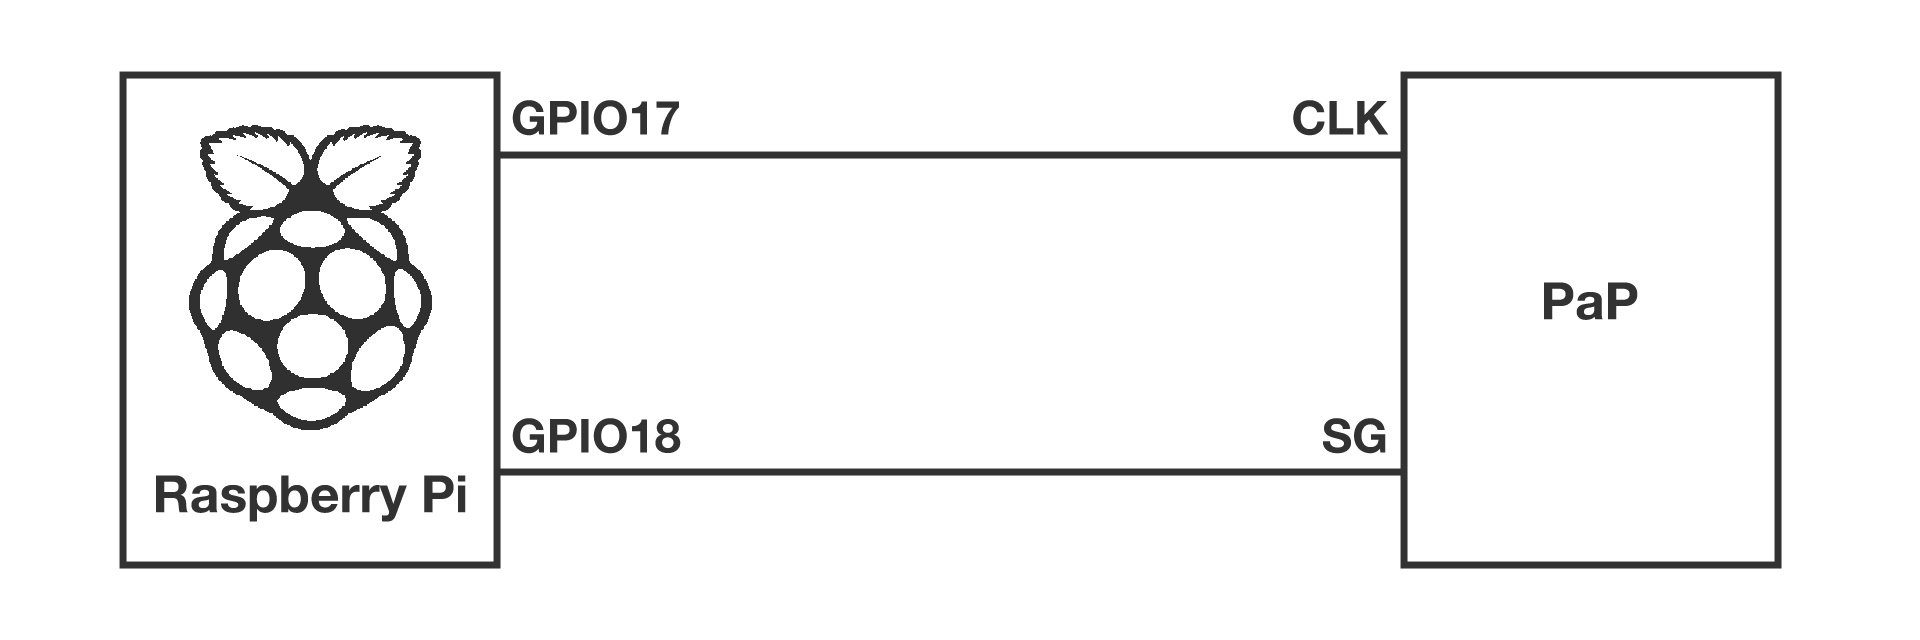
\includegraphics[width=.9\textwidth]{dcpap}
					\caption*{Esquema de conexión entre la Raspberry y el motor PaP. CLK corresponde a la entrada de reloj y SG a la entrada que determina el sentido de giro.}
				\end{center}
			\end{figure}
			\item \textbf{Estime la precisión del PaP y deduzca el número de piñones que tiene este motor.}
			
			Sabiendo que la frecuencia del motor es de aproximadamente 50 Hz (es decir, que en un segundo se dan 50 pasos) y que esto resulta en una velocidad de 1 vuelta por segundo, no es difícil llegar a la conclusión:
			
			$$ 50 \dfrac{\text{pasos}}{\text{segundo}} \cdot 1 \dfrac{\text{segundo}}{\text{vuelta}} = 50 \dfrac{\text{pasos}}{\text{vuelta}} $$
			
			Nos salen aproximadamente 50 pasos (o piñones) por vuelta, resultando en una precisión de 7.2º. Esto no dista mucho del valor tabulado, que son 47 pasos/vuelta, que tiene una precisión de 7.7º.
			
			\item \textbf{Conecte la señal de reloj y la señal de sentido de giro a sendas salidas de la RaspBerry. Compruebe que puede mover el motor en ambos sentidos.}
			
			Comprobado.
			
			\item \textbf{Haga un pequeño programa que dado un ángulo de giro por pantalla, mueve el motor PaP a esa orientación.}
			\begin{verbatim}
				#include <wiringPi.h>
				#include <stdio.h>
				#include <softPwm.h>
				
				#define PAP_CLK 0
				#define PAP_SG 1
				#define DIENTES 47
				
				int main(){
				    int ang=0,howmuch,dif;
				    
				    wiringPiSetup();
					pinMode(PAP_CLK,OUTPUT);
					pinMode(PAP_SG,OUTPUT);
					softPwmCreate(PAP_CLK, 0, 100);
				
				
				    printf("¿A cuántos grados quieres ponerte?\n");
				    while(){
				        scanf("%d",&howmuch);
				        dif = howmuch-ang;
				        
				        softPwmWrite(PAP_CLK,150); //activamos el PWM
				        delay(20*dif*DIENTES/360);//esperamos una cantidad de tiempo adecuada (20ms*nº periodos necesarios)
				        softPwmWrite(PAP_CLK,0); //apagamos el PWM
				        
				        ang = howmuch;
				        printf("\n Maravilloso. ¿A cuántos grados quieres ponerte ahora?\n");
				    }
				}
			\end{verbatim}
			
		\end{enumerate}

\subsection{Sesión 2}
	\begin{enumerate}[(a)]
			\item \textbf{Vea qué rango de valores de PWM sirven para girar en un sentido u otro. Escoja dos valores para usar dos velocidades (alta y baja). Encuentre el valor de PWM necesario para que el motor (o la rueda) no se mueva. Estos valores serán utilizados en el futuro.}

			Usando un rango de 100 (lo que equivale a un periodo de 10 ms), encontramos que para valores mayores de 15 (1.5 ms) los motores giraban en un sentido y para menores de 15 lo hacían en el otro. No cuesta ver que para un valor de 15 (1.5 ms) los motores se quedan (casi) parados.
			
			No se encontraron diferencias significativas en las velocidades de los motores para diferentes valores del PWM más allá del cambio de sentido de giro que ya hemos comentado.
			
			\item \textbf{Verifique que es capaz de mover el motor en ambos sentidos.}
			
			Sí, el motor puede moverse en ambos sentidos y el sentido puede cambiarse modificando el \textit{duty cicle} del PWM.
			
			\item \textbf{Calibre las vueltas por segundo que da el motor en función de los pulsos generados (velocidad escogida).}
			
			\begin{center}
			\begin{tabular}{ c | c c }
			 \textbf{Velocidad de giro (rps)} & \textbf{Motor 1} & \textbf{Motor 2} \\ 
			 \hline
			 \textbf{Sentido horario} & 0.8365 & 0.9208 \\  
			 \textbf{Sentido antihorario} & 0.8421 & 0.8606  
			\end{tabular}
			\end{center}
		\end{enumerate}
		
	\section{Diseño del robot}
	
	Más abajo se pueden ver fotografías del montaje del robot. No se han añadido mejoras significativas de ningún tipo más allá de la búsqueda de la disposición óptima de los elemento en cuanto a la distribución de peso y la simplicidad del cableado.
	
	\begin{figure}[htbp]
	\centering
	{\begin{minipage}{0.31\linewidth}
		\centering
		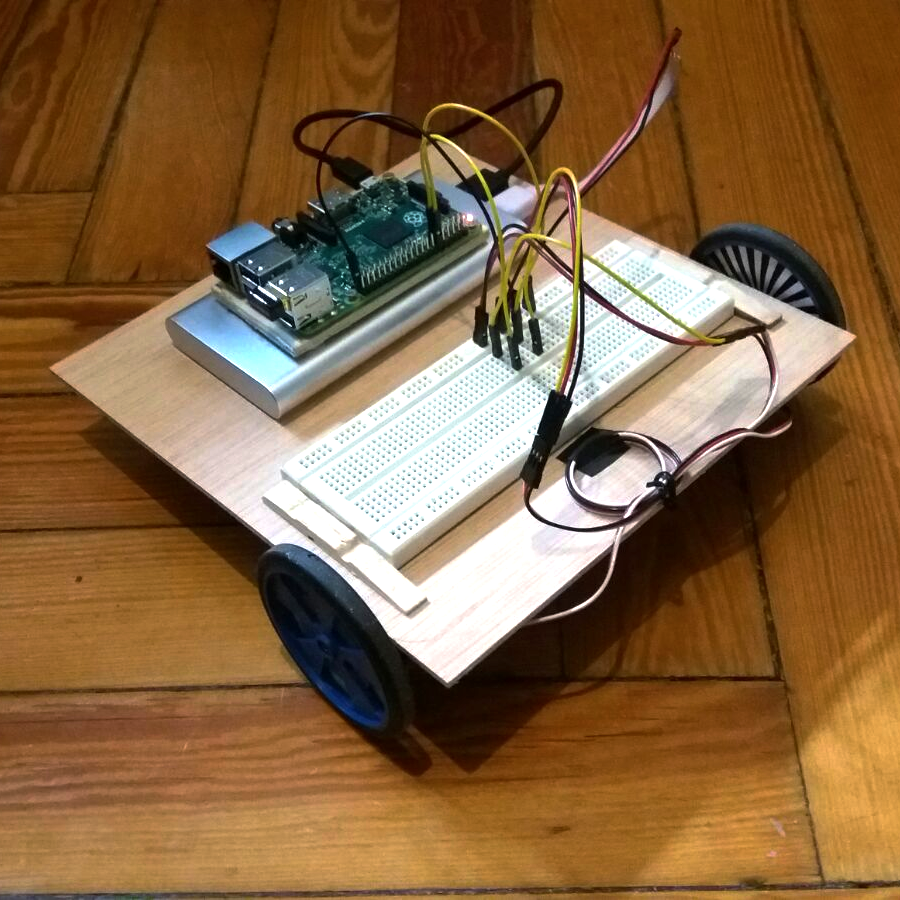
\includegraphics[width=\textwidth]{robglob}
		\subcaption{Fotografía general del robot. Se puede apreciar la distribución de cables y elementos.}
	\end{minipage}
	\hfill
	\begin{minipage}{0.31\linewidth}
		\centering
		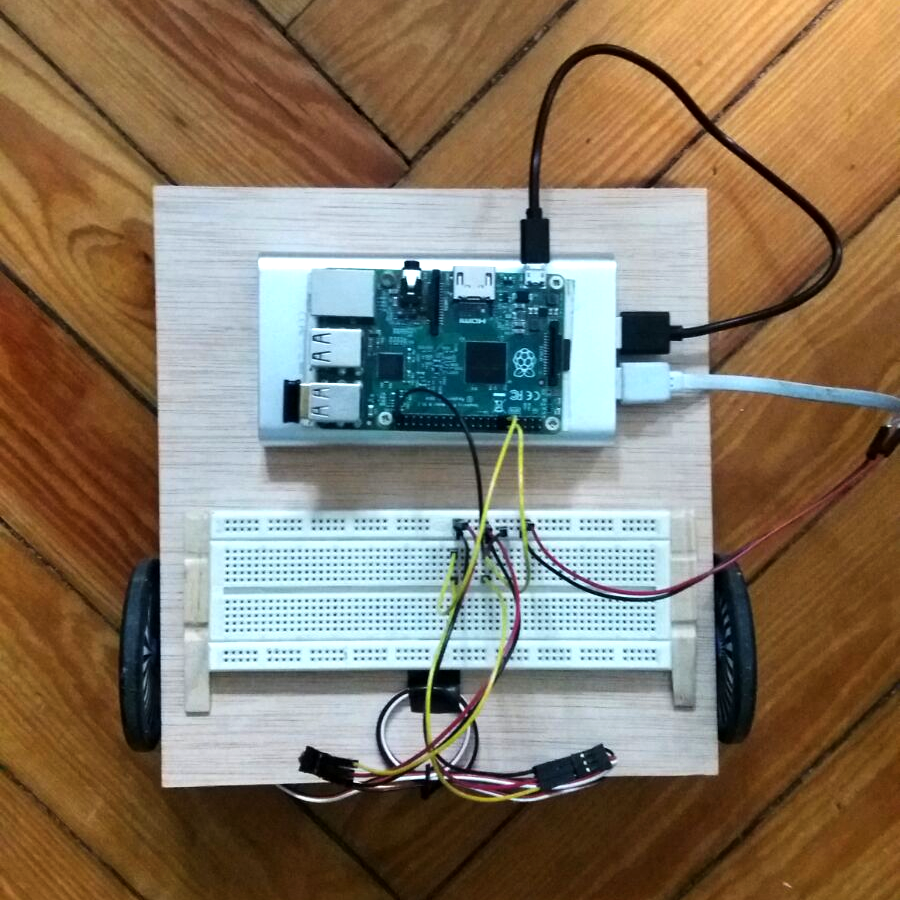
\includegraphics[width=\textwidth]{robtop}
		\subcaption{Vista superior del robot. Se aprecian la \textit{protoboard}, la Raspberry y la batería externa.}
	\end{minipage}
	\hfill
	\begin{minipage}{0.31\linewidth}
		\centering
		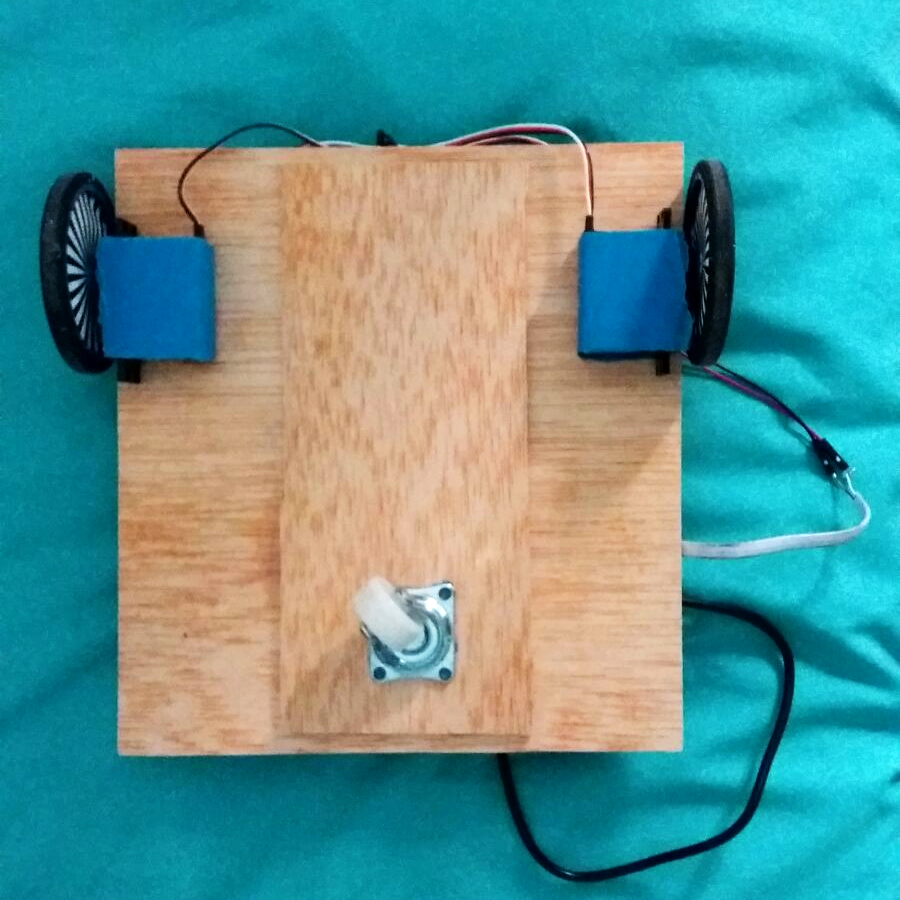
\includegraphics[width=\textwidth]{robbot}
		\subcaption{Vista inferior del robot. Se aprecian las ruedas, los servos y el \textit{roll on}.}
	\end{minipage}}
\end{figure}

\section{Control de los motores}
Para controlar los motores hemos usado el código del archivo move.c.

\begin{verbatim}
#include <wiringPi.h>
#include <softPwm.h>

/* Definimos todas las especificaciones del robot */
#define INIVAL 0 // Valor inicial del PWM
#define RANGO 100 // Rango del PWM
#define PINR 0 // Pin para la rueda derecha
#define PINL 1 // Pin para la rueda izquierda
#define PERIIZQ 0.22 // Perímetro (en m) de las ruedas.

//Qué valores pasar al PWM y demás cosis.
#define FWL 20
#define FWR 5
#define BKL 10
#define BKR 25

//Vueltas/segundo de cada rueda
#define FWLV 0.860585
#define FWRV 0.8365
#define BKLV 0.9208
#define BKRV 0.8421

//Vueltas/segundo del giro global
#define SPIN 0.326 //rev/s
//Velocidad (grosso modo) de avance del robot.
#define SPEED 0.174 //m/s
//s/vuelta pivotando
#define PIVL 7.52
#define PIVR 7.2

//Para.
void stop(){
    softPwmWrite(PINL,0);
    softPwmWrite(PINR,0);
}

//Va hacia delante N metros. N<0 -> hacia atrás.
void go(float metros){
    unsigned int tim=0; //tiempo que tardaremos (grosso modo) en recorrer los metros
    int left=0, right=0; //marchas de las ruedas
    
    if(metros > 0){
        left = FWL;
        right = FWR;
    } else {
        left = BKL;
        right = BKR;
        metros = -metros;
    }
    tim = metros*1000/SPEED;
    
    if(metros!=0){
        softPwmWrite(PINL,left);
        softPwmWrite(PINR,right);
        delay(tim);
        stop();
    }
}

//Gira un cierto ángulo
void turn(float ang){
    int mchl=0, mchr=0; //marchas izquierda y derecha
    unsigned int tim=0;
    
    //ang > 0 hacia la derecha, ang < 0 hacia la izquierda
    if(ang>0){
        mchl = FWL;
        mchr = BKR;
    } else {
        mchl = BKL;
        mchr = FWR;
    }
    
    tim = ang*1000/(360*SPIN); //luego meteremos el encoder y tal
    
    if(ang!=0){
        softPwmWrite(PINL,mchl);
        softPwmWrite(PINR,mchr);
        delay(tim);
        stop();
    }
}

//Pivota un cierto ángulo
void pivot(float ang){
    int mchl=0, mchr=0; //marchas izquierda y derecha
    unsigned int tim=0;
    float vel=0;
    
    //ang > 0 hacia la derecha, ang < 0 hacia la izquierda
    if(ang>0){
        mchl = FWL;
        vel = PIVR;
    } else {
        mchr = FWR;
        vel = PIVL;
    }
    
    tim = ang*1000*vel*360; //luego meteremos el encoder y tal
    
    if(ang!=0){
        softPwmWrite(PINL,mchl);
        softPwmWrite(PINR,mchr);
        delay(tim);
        stop();
    }
}
\end{verbatim}

Dos comentarios respecto a este código:

\begin{itemize}
	\item Tenemos dos modos de giro: \textit{turn} y \textit{pivot}. \textit{pivot} hace girar al robot alrededor de la rueda interior, mientras que \textit{turn} hace girar al robot alrededor de un punto medio entre las ruedas.
	\item Este código está sujeto a cambios, puesto que aún falta por incorporar el encoder, el cual nos servirá para asegurar que el robot avance recto y se gire exactamente el ángulo que le pedimos.
\end{itemize}
\end{document}